\documentclass[12pt]{ociamthesis}  % default square logo 
%\documentclass[12pt,beltcrest]{ociamthesis} % use old belt crest logo
%\documentclass[12pt,shieldcrest]{ociamthesis} % use older shield crest logo

%load any additional packages
\usepackage{amssymb}

%input macros (i.e. write your own macros file called mymacros.tex 
%and uncomment the next line)
%\include{mymacros}

\title{Panduan Penulisan\\[1ex]     %your thesis title,
        Jurnal Ilmiah}   %note \\[1ex] is a line break in the title

\author{Rolly Maulana Awangga}             %your name
\college{ORCID : 000-0001-5530-9505}  %your college

%\renewcommand{\submittedtext}{change the default text here if needed}
\degree{Politeknik Pos Indonesia}     %the degree
\degreedate{Bandung 2018}         %the degree date

%end the preamble and start the document
\begin{document}

%this baselineskip gives sufficient line spacing for an examiner to easily
%markup the thesis with comments
\baselineskip=18pt plus1pt

%set the number of sectioning levels that get number and appear in the contents
\setcounter{secnumdepth}{3}
\setcounter{tocdepth}{3}


\maketitle                  % create a title page from the preamble info
\begin{dedication}
`Jika Kamu tidak dapat menahan lelahnya belajar, \\
Maka kamu harus sanggup menahan perihnya Kebodohan.'\\ 
~Imam Syafi'i~\\
\end{dedication}        % include a dedication.tex file
\begin{acknowledgements}
Pertama-tama kami panjatkan puji dan syukur kepada Allah SWT yang telah memberikan rahmat dan hidayah-Nya sehingga PPJI ini dapat diselesaikan.
\end{acknowledgements}   % include an acknowledgements.tex file
\begin{abstract}
	Panduan Penulisan Jurnal Ilmiah (PPJI) ini dibuat dengan tujuan memberikan acuan bagi para sivitas akademika
	yang memulai menulis jurnal ilmiah. Pada intinya PPJI menjelaskan secara lengkap tentang standar pengerjaan jurnal internasional dari pengalaman penulisan dari tahun 2017. Di dalamnya memuat aturan standar penulisan dan penggunaan Latex sebagai editor. Dengan demikian diharapkan semua sivitas akademika dapat membuat jurnal ilmiah dengan
	 lancar dan sesuai dengan standar.
\end{abstract}          % include the abstract

\begin{romanpages}          % start roman page numbering
\tableofcontents            % generate and include a table of contents
\listoffigures              % generate and include a list of figures
\end{romanpages}            % end roman page numbering

%now include the files of latex for each of the chapters etc
\chapter{Standar Perlengkapan}

Dalam pertempuran untuk membuat jurnal ilmiah maka diharapkan memeiliki alat bantu berupa aplikasi. Alat bantu aplikasi tersebut berguna untuk proses mempercepat penulisan jurnal ilmiah. Selain aplikasi juga harus memiliki beberapa akun yang berfungsi untuk memperluas jaringan kolaborasi publikasi ilmiah. Beberapa alat bantu aplikasi dan akun yang wajib dimiliki antara lain :
\begin{enumerate}
\item Grammarly dengan akun premium.
\item akun sharelatex dan latex compiler di komputer.
\item akun researchgate
\item Profile Google Scholar
\item Profile orcid.org
\end{enumerate}
Kemudian yang tidak kalah penting adalah memiliki mentor yang mempunya H-Index diatas 10. Memiliki mentor berfungsi untuk mempercepat proses pematangan diri agar siap produktif membuat jurnal. Lebih bagus lagi mentor dari luar negeri. Diharapkan memiliki minimal 3 mentor dari lintas institusi pendidikan.

\section{Pencarian Topik}
Satu-satunya cara adalah untuk mendapatkan topik publikasi adalah dengan membaca jurnal 5 tahun terakhir terindex scopus minimal sebanyak 15 buah. Carilah jurnal dengan pencarian  kata kunci sesuai dengan topik yang kita inginkan. Kemudian tuangkan dalam slide presentasi dengan satu halaman setiap jurnal terdiri dari judul, masalah, metode, hasil.

\chapter{Standar Penulisan Jurnal}

Penulisan jurnal untuk pemula disarankan menggunakan Latex. Latex memberikan kemudahan dalam mengisi template sesuai dengan tujuan jurnal. Jika sudah menguasai latex, maka format lain menggunakan doc atau docx sangat mudah untuk dilalui. Template latex bisa di unduh pada menu dokumen portal kampus keren. Karena dalam penulisan jurnal format sesuai dengan template merupakan syarat paling mutlak yang dikoreksi pertama kali sebelum di teruskan kepada pada reviewer jurnal. Setelah sampai kepada reviewer, penulisan jurnal harus mengikuti standar penulisan akademis dan mengikuti kerangka jurnal. Jurnal wajib menggunakan bahasa inggris (Amerika) yang dikoreksi bersama mentor atau kolaborator. 

\section{Standar Penulisan}
Di dalam penulisan artikel ilmiah harus mengikuti standar minimal penulisan ilmiah. Standar ini digunakan untuk menyamakan semantik bahasa agar tulisan lebih mudah dibaca dan dipahami. Penggunaan standar merupakan keniscayaan dalam penulisan artikel ilmiah.

\subsection{Penggunaan Kalimat}
Penulisan jurnal harus menggunakan kalimat aktif dan positif. Memiliki Subject, Predikat dan Object yang jelas. Tidak bertele-tele dan terlalu panjang dalam penggunaan kalimat(terlalu banyak kata sambung dan tanda koma). Satu paragraf minimal terdiri dari tiga kalimat. Hindari paragraph yang terdiri dari satu kalimat yang biasanya digunakan untuk penjelasan gambar, rumus atau tabel. Lebih baik digabungkan saja dengan narasi paragraph sebelumnya. Jika memang harus ada penjelasan kalimat, maka kembangkan lagi menjadi narasi satu paragraph utuh. 

Tidak boleh menulis kata ganti orang pertama, kedua dan ketiga. Contoh penulisan kata ganti orang yang dihindari seperti :
\begin{enumerate}
 \item Penulis
 \item Saya
 \item Kami
 \item Mereka 
 \item Beliau
\end{enumerate}
Gunakan kata benda seperti penelitian ini, riset ini. Selain itu jika menggunakan singkatan, pastikan di definisikan satu kali pada awal penggunaan singkatan. Jangan mendefinisikan singkatan lebih dari sekali. Cukup mendefinisikan pada pertama kali menggunakan singkatan, selanjutnya pakai singkatannya saja. 

Contoh : Penelitian Mengenai Social Netwprk Analisys (SNA) membawa dampak terhadap pola pemberitaan. SNA memiliki konsep grap yang berkaitan antara satu node dengan node lainnya. Centrality merupakan salah satu konsep SNA untuk memperhitungkan tingkat kepentingan sebuah node.

Format singkatan yang lazim digunakan adalah kepanjangan terlebih dahulu kemudian didalam kurung merupakan singakatannya, hindari melakukan kebalikannya. 
\begin{itemize}
\item Contoh yang benar: Kepanjangan Dari Singkatan (KDR). 
\item Hindari : KDR (Kepanjangan Dari Singkatan).
\end{itemize}

\subsection{Penempatan Sitasi}
Sitasi ditempatkan tepat pada akhir kata atau kalimat penjelasan referensi sebelum tanda 
pemisah antar kalimat (koma atau titik) tanpa spasi. 
Sitasi juga dapat ditumpuk pada sebuah kata atau kalimat yang merupakan  penjelasan singkat dari referensi. 
Please ensure that: all references have been cited in your text. Each citation should be written in the order of appearance in the text. The references must be presented in numbering. Gunakan sitasi latex \verb|\cite{ref}| jika menggunakan latex atau menggunakan aplikasi Mendeley jika menggunakan Word. Contoh penggunaan sitasi :
\begin{itemize}
\item Perhitungan Social Network Analysis(SNA) salah satunya dengan teori graph[1].
\item Komputasi terdiri dari matematika[1] dan perhitungan[2].
\item Kasus yang terjadi pada penguraian bakteri bisa dicermati dengan menggunakan mikroskop[1][2].
\end{itemize}

\subsection{gambar, rumus, tabel}
Pemanfaatan instrumen pendukung gambar kualitasnya harus ditingkatkan, jangan sampai terdapat gambar yang tidak bisa terbaca tulisannya.
Tidak diperbolehkan memberikan narasi penunjukan relatif. seperti :
\begin{itemize}
	\item Lebih detailnya lihat gambar di bawah ini
	\item Untuk lebih jelasnya lihar rumus di bawah ini
	\item data bisa dilihat di tabel di atas
\end{itemize}
Diperbaiki yang seharusnya :
\begin{itemize}
	\item Pada gambar 1.1 terlihat bahwa hasil perhitungan penduduk sudah mulai jenuh.
	\item Total kejenuhan hasil kalkulasi terlihat di tabel 1.1.
	\item Rumus 1.1 merupakan rumus kalkulasi tingkat kejenuhan.
\end{itemize}
Prepare your figures in high quality and created by yourself (not copy and paste from other parties). All legends, captions, etc in your figures MUST in English.


\section{Kerangka Jurnal}
Kerangka acuan dalam membuat jurnal harus memenuhi standar acuan di sub bab ini. Masing-masing kerangka jurnal harus memenuhi standar dan aturan yang ditetapkan. Pengerjaan jurnal biasanya lebih awal daripada pengerjaan laporan.Bagian-bagian dari jurnal terdiri dari abstrak (Abstract), pendahuluan (Introduction), metode (Methods), Penelitian Terkait (Related Works),percobaan (Experiment), hasil (Result) dan diskusi (Discussion).

\subsection{Judul}
Maksimal 10 (sepuluh) kata dalam Bahasa Inggris ringkas dan tegas.

\subsection{Abstract}
Terdiri dari 150-200 kata tanpa ada sitasi. Berisi latar belakang, tujuan,metode, hasil,kesimpulan dan saran. Pada abstrak harus dimunculkan persoalan utama dan pentingnya melakukan penelitian ini, serta solusi yang diusulkan. Isi tertuang dengan kalimat yang jelas.Kata kunci atau keyword ditentukan dengan nama metode yang digunakan dan sub sub bidang penelitian yang dilakukan. Kata kunci minimal harus terdapat lima kata kunci.

\subsection{Introduction}
Pada bagian pendahuluan uraikan rincian persoalan terkini berdasarkan beberapa referensi dari jurnal intenasional yang di sitasi, sehingga penelitian ini layak dilakukan. An Introduction should contain the following three parts:
\begin{itemize}
    \item Background: Authors have to make clear what the context is. Ideally, authors should give an idea of the state-of-the art of the field the report is about.
    \item  The Problem: If there was no problem, there would be no reason for writing a manuscript, and definitely no reason for reading it. So, please tell readers why they should proceed reading. Experience shows that for this part a few lines are often sufficient.
    \item The Proposed Solution: Now and only now! - authors may outline the contribution of the manuscript. Here authors have to make sure readers point out what are the novel aspects of authors work.
\end{itemize}
Authors should place the paper in proper context by citing relevant papers. Setiap ada pemaparan data, informasi, dan sebuah pernyataan pada sebuah kalimat maka wajib diakhiri dengan sitasi.Minimal terdapat sitasi pada setiap kalimat pernyataan, informasi, dan data pada bagian Introduction dari jurnal 5 tahun terakhir terindex scopus.

\subsection{Related Works}
Penjelasan singkat dengan sitasi dari artikel yang direferensikan minimal dari 10 artikel. Artikel yang dijelaskan merupakan artikel yang terkait dengan kata kunci penelitian. Minimal 3 Paragraph. Pada paragraph terakhir harus ada pernyataan perbedaan antara penelitian yang akan dilakukan dengan penelitian yang disebutkan pada sitasi di related works.

\subsection{Method}
Penjelasan teknis yang jelas dan gamblang mengenai metode yang digunakan dengan sitasi. Terdiri dari definisi, konsep, rumus atau diagram. Metode yang digunakan adalah metode yang terdapat pada referensi dalam 5 tahun terakhir  dari  jurnal  internasional  terindex  scopus. 

\subsection{Experiment}
Data sumber yang jelas dan cukup untuk dijadikan penelitian, disertai dengan hasil nya sesuai langkah-langkah yang di tuliskan di Method.

\subsection{Result and Discussion}
Sangat jelas relevasinya dengan latar belakang dan pembahasan, dirumuskan dengan singkat. The presentation of results should be simple and straightforward in style. You should improve your analyzing and also present the comparison between performance of your approach and other researches. Results given in figures should not be repeated in tables. This section report the most important findings, including results of analyses as appropriate. It is very important to prove that your manuscript has a significant value and not trivial.

\subsection{Reference}
Semua  referensi  yang  digunakan  harus  terindex  pada  google  scholar.   Minimal  15 referensi dari jurnal terindeks Scopus dan merupakan artikel dalam 5 tahun terakhir. Jurnal yang terindex scopus bisa dicek di situs scimagojr.com.  Format referensi yang disikan  pada  formulir  pengajuan  penelitian  tingkat  akhir  adalah  BibTex.   BibTex referensi bisa didapatkan pada laman Google Scholar. Gunakan format bibtex dari google scholar, jika anda tidak menggunakan Latex maka gunakan aplikasi Mendeley untuk membuat daftar pustaka atau referensi.

\section{Standar Format Latex}
Beberapa Aturan yang harus dipatuhi :
\begin{enumerate}

    \item file disimpan dalam format ber ekstensi .tex per chapter masing2 di folder section

    \item gambar disimpan dalam folder figures dengan namagambar

    \item referensi dari google scholar,scholar.google.com

    \item Setiap referensi yang diambil, maka tambahkan dan tuliskan ke dalam file bernama references.bib yang berisi kumpulan bibTex dari referensi. Gunakan standar pengutipan yang baik dan benar

    \item Gambar disebutkan di dalam artikel dengan format sesuai labelnya yaitu \\ \verb|\ref{labelgambar}|. \\ Gambar diselipkan dengan menambahkan blok sintaks :
    \begin{verbatim}
    \begin{figure}[ht]
    \centerline{\includegraphics[width=1\textwidth]
    {figures/namagambar.JPG}}
    \caption{penjelasan keterangan gambar.}
    \label{labelgambar}
    \end{figure}
    
    Contoh :
    Pada gambar \ref{labelgambar} dijelaskan bahwa 
    sistem operasi memiliki 3 versi.
    \end{verbatim}

    \item Referensi disebutkan dengan menyebutkan nama di dalam file bibtex No.4. \\
    Contoh, Jika Bibtex sudah diinputkan kedalam reference.bib seperti ini :
    \begin{verbatim}
    @inproceedings{ganapathi2006windows,
      title={Windows XP Kernel Crash Analysis.},
      author={Ganapathi, Archana and Ganapathi, 
      Viji and Patterson, David A},
      booktitle={LISA},
      volume={6},
      pages={49--159},
      year={2006}
    }
    \end{verbatim}
    Maka penulisan kalimat di jurnal : \\
    Dalam sebuah artikel dari Ganapathi yang 
    menyebutkan bahwa komputasi adalah keniscayan \verb|\cite{ganapathi2006windows}|.
    
    \item Penyebutan subbab dan subsubbab diatur dengan cara : \\
    judul sub bab : \\ 
    \verb|\section{nama sub bab}| \\
    judul sub sub bab ditulis dengan :\\ 
    \verb|\subsection{judul sub sub bab} | \\
    judul sub sub sub bab ditulis dengan : \\ \verb|\subsubsection{Judul sub sub sub bab} | \\
    contoh :
    \begin{verbatim}
    \section{Sejarah Peta}
Perkembangan peta dunia tidak luput dari para ahli 
geografi dan kartografi. Peta dunia yang populer pada saat 
ini merupakan 
kontribusi dari para 
pembuat peta sebelumnya

\subsection{Ptolemy's}
Ptolemy's diduga membuat peta pada abad ke 2
\end{verbatim}
    
    \item untuk list dan nomor gunakan enumerate atau itemize contoh :
    \begin{verbatim}
berikut nama anggota kelompok
\begin{enumerate}
\item darso
\item karyo
\item doyok
\end{enumerate}

\begin{enumerate}
\item
This is the first item in the numbered list.

\item
This is the second item in the numbered list.
\end{enumerate}

\begin{itemize}
\item
This is the first item in the itemized list.

\item
This is the first item in the itemized list.
This is the first item in the itemized list.
This is the first item in the itemized list.
\end{itemize}

\begin{itemize}
\item[]
This is the first item in the itemized list.

\item[]
This is the first item in the itemized list.
This is the first item in the itemized list.
This is the first item in the itemized list.
\end{itemize}
    \end{verbatim}
    
    \item spesial karakter menggunakan tanda `\verb|\|' didepannya contoh :
    \begin{verbatim}
\& 
\% 
\$ 
\#  
\{ \}
\_
\"dalam petik\"
`dalam petik'
jika spesial karakter menjadi banyak atau satu baris gunakan verb
contoh :
\verb|%$'%&$&'%'%'%&'%|
    \end{verbatim}
    
    \item untuk tabel gunakan table , dan jangan lupa tabel di referensikan pada kalimat berdasarkan labelnya. contoh:
    \begin{verbatim}
ini merupakan contoh tabel \ref{table:contoh} ukuran kecil.
\begin{table}[h]
\caption{Small Table}
\centering
\begin{tabular}{ccc}
\hline
one&two&three\\
\hline
C&D&E\\
\hline
\end{tabular}
\label{table:contoh}
\end{table}
    \end{verbatim}
    
    \item untuk rumus gunakan tag equation dan di referensikan pada kalimat dengan tag ref sesuai labelnya contoh:
    \begin{verbatim}
Luas permukaan dijelaskan pada rumus \ref{eq:1}.Volume dijelaskan 
pada rumus \ref{eq:2}.
$L$ merupakan luas, $\pi$ adalah 3,14.
\begin{equation}\label{eq:1}
     L = 4 \pi r^2 \,
\end{equation}
 \begin{equation}\label{eq:2}
     V = \frac{4}{3}\pi r^3
\end{equation}
    \end{verbatim}
    
    \item untuk kode program menggunakan verbatim
    \begin{verbatim}
\ begin{verbatim}
a = "anu"
b = "itu"
c = a + b
print(c) 
\ end{verbatim}
    \end{verbatim}
\end{enumerate}





\chapter{Penutup}

Jika anda sudah siap untuk melakukan publikasi silahkan lakukan publikasi pada jurnal yang terdapat pada scimagojr.com.

%now enable appendix numbering format and include any appendices
\appendix
\chapter{Latex Symbol}
Berikut adalah daftar pemakaian simbol dalam latex
\begin{enumerate}
	\item The Comprehensive LATEX Symbol List : \\
	\verb|http://tug.ctan.org/info/symbols/comprehensive/symbols-a4.pdf|
	\item List of Math Symbol : \\
	\verb|https://oeis.org/wiki/List_of_LaTeX_mathematical_symbols|
	\item List of Latex Symbol : \\
	\verb|http://latex.wikia.com/wiki/List_of_LaTeX_symbols|
\end{enumerate}
\chapter{Contoh Penilaian Reviewer Jurnal}

gambar \ref{form1} dan \ref{form2} merupakan contoh bagaimana reviewer menilai jurnal kita. 
\begin{figure}[ht]
      \centerline{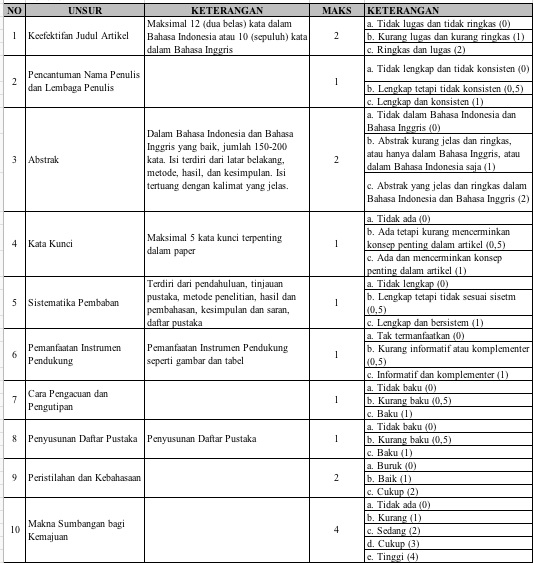
\includegraphics[width=1\textwidth]
      {figures/form1}}
      \caption{Form nilai bagian 1.}
      \label{form1}
      \end{figure}

	\begin{figure}[ht]
	      \centerline{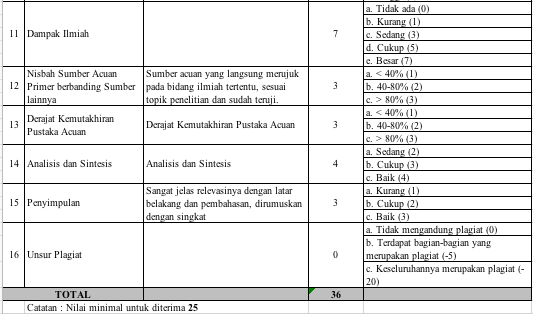
\includegraphics[width=1\textwidth]
	      {figures/form2}}
	      \caption{form nilai bagian 2.}
	      \label{form2}
	      \end{figure}


%next line adds the Bibliography to the contents page
\addcontentsline{toc}{chapter}{Bibliography}
%uncomment next line to change bibliography name to references
%\renewcommand{\bibname}{References}
\bibliography{references}        %use a bibtex bibliography file refs.bib
\bibliographystyle{plain}  %use the plain bibliography style

\end{document}

